\section{Vandfaldsmetoden}\label{sec:vandfald}
Vandfalds-modellen er en sekventiel procesmodel som består af 5-7 forskellige faser. 
Navnet vandfald er blevet brugt, da det ikke er muligt at vende tilbage til foregående faser, 
når først en fase er færdiggjort. Resultatet fra hver fase er et krav for at kunne starte på den næste. 
Hvis kunden kommer med store ændringer til kravene, bliver hele processen nødt til at starte forfra.  
Vandfalds-modellen kan ses på Figur \ref{fig:waterfallmodel} \\

\begin{figure}[h]
    \centering
    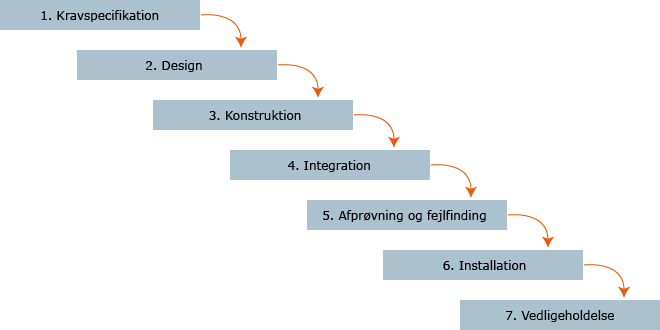
\includegraphics[width=0.7\textwidth]{figures/waterfall.png}
    \caption{Vandfaldsmodellen \cite{WaterfallModel}}
    \label{fig:waterfallmodel}
\end{figure}

Denne metode kan virke godt I forbindelse med mindre projekter, hvor det afsluttende produkt er 
helt defineret og det ikke forventes at ændringer kan forekomme. Hvis projektet er for stort og kompliceret,
kan det ofte medføre, at der på sigt vil være ændringer i enten arkitekturen eller selve funktionaliteten.
Dette tager vandfaldsmodellen ikke højde for.

\section{Agile metoder}\label{sec:agilemetoder}
Agil er en betegnelse for en række iterative softwareudviklingsmetoder, hvor der løbende leveres små dele af 
produktet til kunden. Agile udviklingsmetoder er oftest kendetegnet ved Det Agile Manifest \cite{AgileManifesto}.
Manifestet beskriver blandt andet hvordan samtaler og møder med kunden, samt god, fungerende software er i fokus, 
fremfor en lang liste af processer og værktøjer og fuldstændig dokumentation. \\

Ved udvikling af større softwaresystemer, hvor kunden er en nær kontakt igennem udviklingsperioden, kan udviklerteamet
drage stor fordel af at udvikle agilt. Dette skyldes at agile metoder bygger på \textit{continual improvement},
hvilket vil sige at produktet bliver udviklet inkrementelt, sådan at man altid har noget at vise kunden. Desuden er en fordel ved agile
metoder, at de er omstillingsparate. Dette skyldes at man kun planlægger sit arbejde få uger frem.